\section{Introduction}
In this research, we deal with human-humanoid cooperative-manipulation tasks of large deformable objects where simultaneous operations by two individuals are required. So far, we made a presentation on cooperative operations of large objects with the aim of acquiring the motion of the robot by imitating that of the human~\cite{h-ito:ROBOMEC2018}. While a motion capture device was attached to the human body to acquire human motion, there were some difficulties remained:
\begin{itemize}
  \item the sensors can be lost when occlusion occurred during the object manipulation,
  \item the work space are limited due to the recognizable range of the sensors.
\end{itemize}

Therefore, in this paper, to acquire the autonomous arm motion of the robot during the task, the target coordinates of the hand are decomposed into two elements: the target position and the target orientation. The former is derived by imitating the human hand movement and the latter by introducing the potential field of the object. Eventually, by combining them, the target coordinates of robot hands are determined. With applying our proposed method, we conducted some experiments with a life-sized humanoid robot HRP-2 and confirmed its effectiveness.

%% \begin{figure}[htbp]
%%  \begin{center}
%%   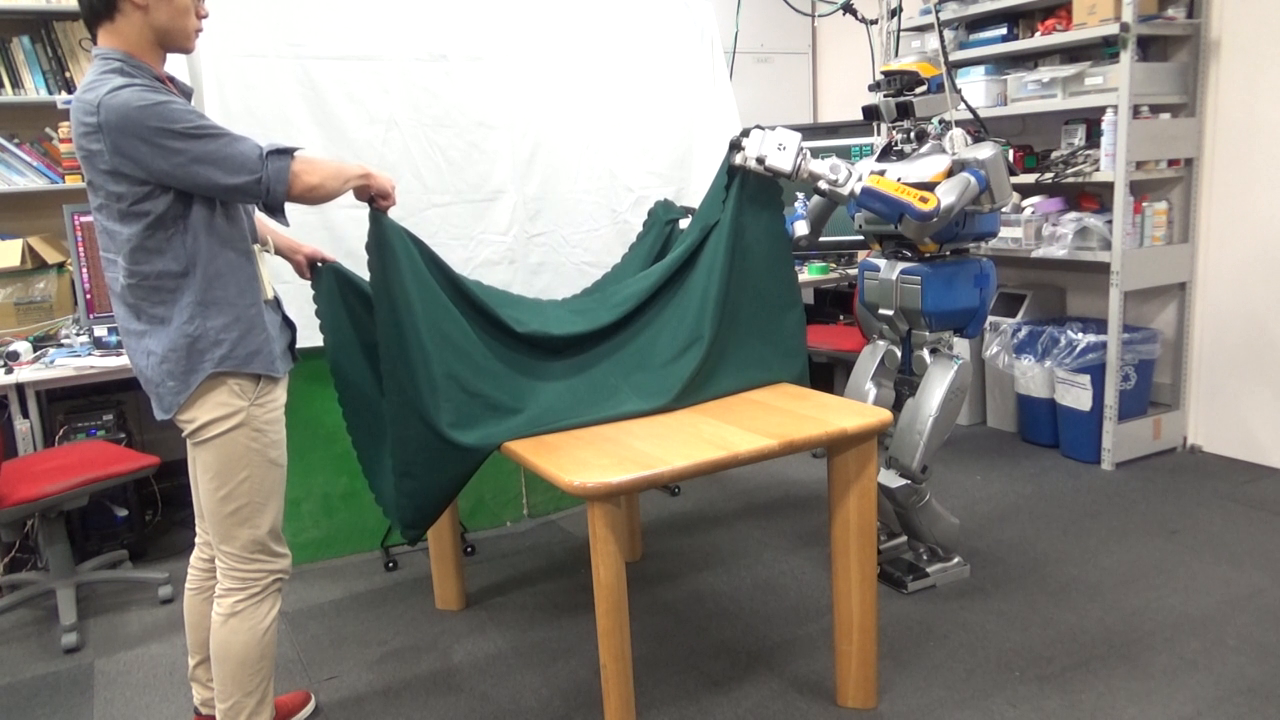
\includegraphics[width=0.80\columnwidth]{figs/fold-top.png}
%%   \caption{}
%%   \label{figure:system}
%%  \end{center}
%%  \vspace{-5mm}
%% \end{figure}
